\section{Delay \& Sum Algorithmus}

	Der Delay \& Sum Algorithmus ist eine Möglichkeit, eine akustische Antenne zu implementieren. Der Algorithmus beruht auf der Addition ("Sum") der unterschiedlich verzögerten ("Delay") Eingangssignale der einzelnen Mikrofone. Dabei müssen ebene Schallwellen und Kugelschallwellen jeweils unterschiedlich behandelt werden. Generell gilt die Annahme, dass sich Antenne und Quelle im Freifeld befinden (keine Reflexionen).
	
	%Skizze generell
	In Abbildung \ref{fig:das_basic} ist ein beispielhaftes Mikrofonarray dargestellt, bestehend aus $N$ Mikrofonen $m_1,...,m_N$, die im Abstand von $\Delta x$ in einer Reihe angeordnet sind. Eine Schallquelle $Q$ befindet sich im Winkel $\alpha$ vor dem Array.
	Dieser Winkel führt dazu, dass die Schallwelle jedes Mikrofon mit einer bestimmten Verzögerung $\tau_n$ erreicht.
	Die Summe der Mikrofonsignale $p_n(t)$ ist dann
	\begin{equation}
		s_{sum}(t, \alpha) = \sum_{n=1}^{N} p_n(t - \tau_n(\alpha))
	\end{equation}
	Unter der Annahme, dass der Übertragungsweg von der Quelle zur Summierstelle (Luft, Mikrofon, Kabel) keine Signalveränderungen bewirkt, wird also das selbe Signal mit $N-1$ zeitlich verschobenen Kopien von sich selbst addiert.
	Dadurch kommt es zu Auslöschungen und Abschwächungen, sodass generell $RMS(s_{sum}(t, \alpha=0)) \ge RMS(s_{sum}(t, \alpha \ne 0))$.
	
	Die Idee des Delay \& Sum Algorithmus ist nun, die theoretischen Verzögerungszeiten für alle Winkel $\alpha \in [-90^{\circ}, 90^{\circ}]$ zu berechnen und durch nachträgliches "inverses" Verzögern der Mikrofonsignale auszugleichen.
	Anschließend berechnet man von diesen "invers verzögerten" Signalen den Effektivwert und sucht den Winkel, unter dem dieser maximal wurde.
	Dieser Winkel wird dann als Schalleinfallsrichtung angenommen.
	
	\begin{figure}[h]
		\begin{center}
		\includegraphics[scale=0.3]{img/DelaySumDiagram}
		\caption{Beispielhaftes Mikrofonarray mit 8 Mikrofonen}
		\label{fig:das_basic}
		\end{center}		
	\end{figure}

\subsection{Delay \& Sum für Ebene Wellen}
	
	Eine Ebene Welle zeichnet sich dadurch aus, dass ihre Wellenfront eine Ebene ist. Die Ausbreitungsrichtung ist also überall gleich.
	Grundsätzlich strahlen "kleine" Quellen (wie zum Beispiel ein Mensch oder ein Lautsprecher) Schall kugelförmig ab. Mit zunehmender Entfernung von der Quelle ähnelt die Schallwelle jedoch immer mehr einer ebenen Welle, sodass ab einer gewissen Distanz von der Schallquelle auch die Annahme einer ebenen Wellenausbreitung getroffen werden kann.
	
	%Skzze ebene Wellen
	Für ebene Wellen stellt sich der Delay \& Sum Algorithmus recht einfach dar. Trifft eine ebene Welle unter dem Winkel $\alpha$ auf das Mikrofonarray, so trifft diese zuerst auf das äußerste Mikrofon und erreicht alle anderen Mikrofone erst nach einer gewissen Verzögerungszeit $\tau_n$.
	Dabei ist speziell für die Annahme ebener Wellen $\tau_n = (n - 1) * \Delta t$. Die Verzögerungszeit zwischen zwei Mikrofonsignalen $\Delta t$ kann mit 
	\begin{equation}
		\Delta t = \frac{\Delta x}{c} = \frac{\Delta x \cdot \sin(\alpha)}{c}
	\end{equation}
	berechnet werden, wobei $c = 340 \frac{m}{s}$ für die Schallgeschwindigkeit in Luft angenommen wird.
	Das Ausgangssignal des Arrays für einen Winkel $\alpha$ berechnet sich dann mit
	\begin{equation}
		s = \sqrt{\frac{1}{T} \int_{0}^{T} \sum_{n=1}^{N} p_m(t - \tau_n(\alpha))}
		\label{eq:das_plane} \footnote{Möser (Hrsg.), Messtechnik der Akustik, Springer 2010, S. 366f}
	\end{equation}
	
	Trägt man den Effektivwert des Arraysignals über dem Winkel auf, so ergibt sich die Richtungsfunktion des Arrays. In Abbildung \ref{fig:bsp_plot} ist beispielhaft die Richtungsfunktion für eine Quelle bei $\alpha = 15^{\circ}$ dargestellt.
	Das Maximum der Effektivwerte ist deutlich bei 15\textdegree\ erkennbar.
	
	\begin{figure}[h]
		\begin{center}
			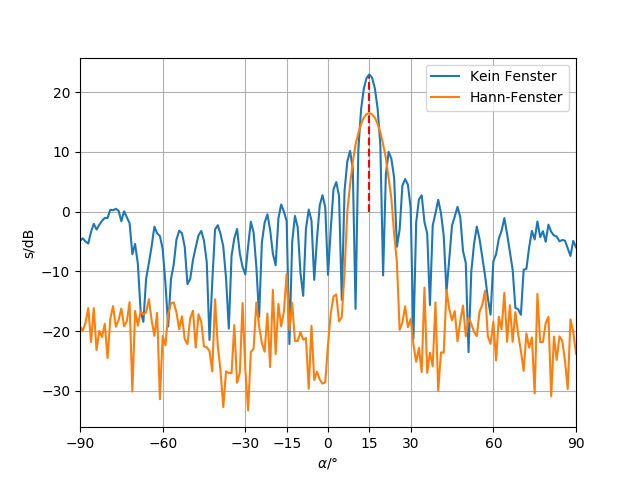
\includegraphics[scale=0.7]{img/bsp_plot_15_beides.png}
			\caption{Richtungsfunktion für eine Quelle bei $\alpha=15^{\circ}$ mit und ohne Gewsichtung. \\
				Das Quellsignal ist ein Sinus mit $f=1000Hz$, das Array hat 20 Mikrofone mit $\Delta x = 0.2m$.}
			\label{fig:bsp_plot}
		\end{center}
	\end{figure}

\subsection{Gewichtung der Mikrofone}

	Die Richtungsfunktion lässt sich durch eine Gewichtung der einzelnen Mikrofonsignale verschieden formen. In Abbildung \ref{fig:bsp_plot} ist im Vergleich eine Richtungsfunktion mit und ohne Gewichtung zu sehen.
	Zur Gewichtung der Mikrofone wurde hier die Hann-Fensterfunktion verwendet. Man erkennt, dass das Hauptmaximum deutlich verbreitert wurde, während die Nebenmaxima abgesenkt wurden.
	Allgemein ergibt die Richtungsfunktion mit Gewichtung geringere Werte als ohne.
	Dies resultiert aus der Absenkung der einzelnen Mikrofonsignale durch die Fensterfunktion.
	Je nach Anwendungsfall empfehlen sich verschiedene Fensterfunktionen. Sollen zum Beispiel mehrere Quellen, die eng beieinander liegen, erkannt werden, so wird ein schmaleres Hauptmaximum benötigt\footnote{Möser (Hrsg.), Messtechnik der Akustik, Springer 2010, S. 374ff}.